\subsection{O Método Beam-Warming}

O método de Beam-Warming pode ser considerado um método do tipo Upwind de segunda ordem. Para esse método, os fluxos são determinados mediante a adição de um termo extra aos fluxos do método Upwind de primeira ordem:

\begin{equation}
F_{i+1/2}^n = \bar{u} Q_i^n + \bar{u} \left(1 - \frac{\bar{u} \Delta t}{2 \Delta x}\right) (Q_i^n - Q_{i-1}^n)
\end{equation}

\begin{equation}
F_{i-1/2}^n = \bar{u} Q_{i-1}^n + \bar{u} \left(1 - \frac{\bar{u} \Delta t}{2 \Delta x}\right) (Q_{i-1}^n - Q_{i-2}^n)
\end{equation}

Portanto, a forma geral da atualização de \( Q_i^{n+1} \) para o método Beam-Warming é dada por:

\begin{equation}
Q_i^{n+1} = Q_i^n - C(Q_i^n - Q_{i-1}^n) - C(1 - C)(Q_i^n - 2 Q_{i-1}^n + Q_{i-2}^n)
\end{equation}

\begin{figure}[H]
    \centering
    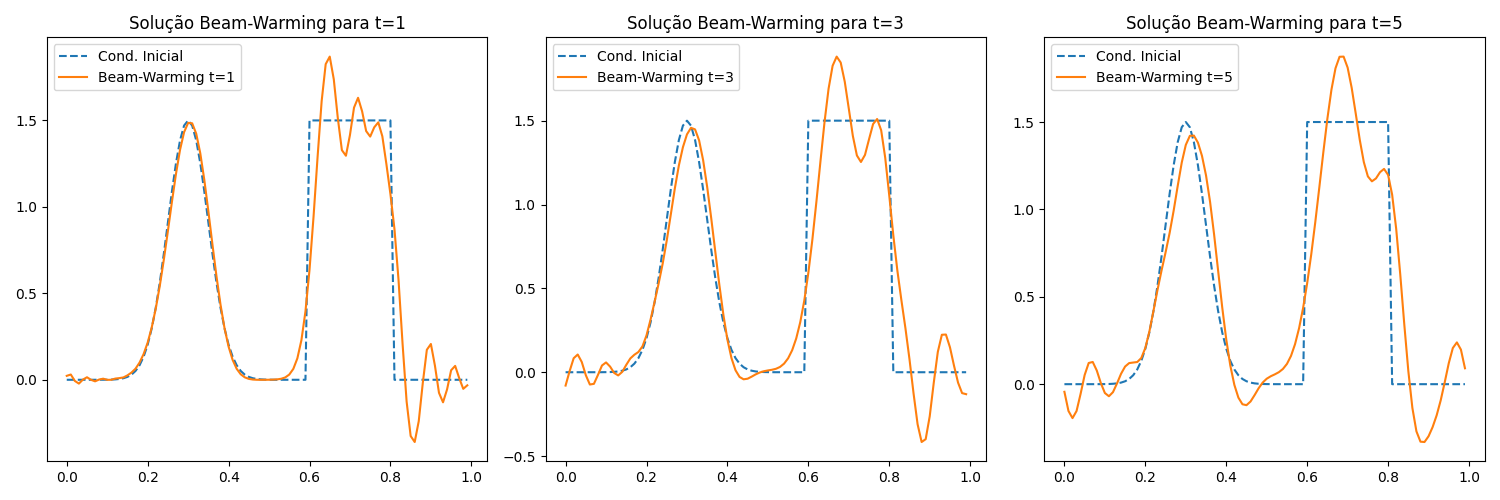
\includegraphics[width=\textwidth]{code/images/Beam-Warming.png}
    \caption{Solução Beam-Warming para $t=1$, $t=3$, e $t=5$, com a condição inicial representada pela linha tracejada.}
\end{figure}

\begin{table}[H]
    \centering
    \begin{tabular}{lrrrrr}
\toprule
 & Posição Espacial & Cond. Inicial & Beam-Warming t=1 & Beam-Warming t=3 & Beam-Warming t=5 \\
\midrule
0 & 0.000000 & 0.000000 & 0.000080 & 0.011905 & 0.055474 \\
1 & 0.050000 & 0.000006 & 0.001377 & 0.023119 & 0.065938 \\
2 & 0.100000 & 0.000503 & 0.014635 & 0.079522 & 0.137594 \\
3 & 0.150000 & 0.016663 & 0.094425 & 0.215688 & 0.270011 \\
4 & 0.200000 & 0.203003 & 0.365367 & 0.445116 & 0.443586 \\
5 & 0.250000 & 0.909796 & 0.836718 & 0.694310 & 0.602054 \\
6 & 0.300000 & 1.500000 & 1.117720 & 0.813352 & 0.673555 \\
7 & 0.350000 & 0.909796 & 0.857233 & 0.711728 & 0.624466 \\
8 & 0.400000 & 0.203003 & 0.371055 & 0.469340 & 0.496815 \\
9 & 0.450000 & 0.016663 & 0.090523 & 0.266608 & 0.388061 \\
10 & 0.500000 & 0.000503 & 0.041207 & 0.241638 & 0.389089 \\
11 & 0.550000 & 0.000006 & 0.236351 & 0.434262 & 0.529188 \\
12 & 0.600000 & 1.500000 & 0.803478 & 0.776761 & 0.758244 \\
13 & 0.650000 & 1.500000 & 1.338980 & 1.102181 & 0.970629 \\
14 & 0.700000 & 1.500000 & 1.472451 & 1.237641 & 1.060403 \\
15 & 0.750000 & 1.500000 & 1.333151 & 1.114042 & 0.978795 \\
16 & 0.800000 & 1.500000 & 0.829878 & 0.791623 & 0.758141 \\
17 & 0.850000 & 0.000000 & 0.235362 & 0.424940 & 0.487426 \\
18 & 0.900000 & 0.000000 & 0.019660 & 0.163072 & 0.257071 \\
19 & 0.950000 & 0.000000 & 0.000293 & 0.043092 & 0.113403 \\
\bottomrule
\end{tabular}

    \caption{Tabela de resultados para o método Beam-Warming nas posições espaciais selecionadas e diferentes tempos}
    \label{tab:beam_warming}
\end{table}

\subsection{Análise dos Resultados do Método Beam-Warming}

O método Beam-Warming é uma extensão de segunda ordem do método Upwind e oferece maior precisão em relação à dissipação. Na Figura, podemos ver que a solução para \( t = 1 \) preserva bem o perfil inicial, com uma redução limitada na amplitude. Para \( t = 3 \) e \( t = 5 \), entretanto, começam a surgir pequenas oscilações em torno das regiões de transição, o que é característico de métodos de segunda ordem sem controle de oscilação. No geral, o método Beam-Warming apresenta uma boa conservação do perfil, mas com leve tendência a oscilações em tempos maiores.

\subsection{Implementação em Python}

O código em Python é utilizado para resolver a advecção com o método Beam-Warming, aplicando condições de contorno periódicas. O código é estruturado com uma função principal \texttt{resolverAdveccao} para calcular a solução da advecção para diferentes métodos numéricos e uma função específica para o método Beam-Warming.

\begin{lstlisting}[language=Python, caption={Código para resolver a advecção usando o método Beam-Warming}, label={lst:codigo_beam_warming}]
# Função para resolver a advecção com diferentes métodos numéricos
def resolverAdveccao(metodo, condicaoInicial, intervaloTempo, intervaloEspacial, numeroCourant, tempoFinal):
    """
    Calcula a solução da advecção para um determinado método e tempo final.
    """
    densidade = condicaoInicial.copy()
    tempoAtual = 0
    while tempoAtual < tempoFinal:
        densidade = metodo(densidade, intervaloTempo, intervaloEspacial, numeroCourant)
        tempoAtual += intervaloTempo
    return densidade

# Método Beam-Warming com condições de contorno periódicas
def metodoBeamWarming(densidade, intervaloTempo, intervaloEspacial, numeroCourant):
    """
    Calcula a solução de advecção usando o método Beam-Warming.
    """
    novaDensidade = densidade.copy()
    for i in range(numPontosEspaco):
        novaDensidade[i] = densidade[i] - numeroCourant * (densidade[i] - densidade[i-1]) - \
                            0.5 * numeroCourant * (1 - numeroCourant) * (densidade[i] - 2 * densidade[i-1] + densidade[i-2])
    return novaDensidade

# Cálculo da densidade para diferentes tempos
densidadeBeamWarming1 = resolverAdveccao(metodoBeamWarming, condicaoInicial, intervaloTempo, intervaloEspacial, numeroCourant, tempoFinal1)
densidadeBeamWarming3 = resolverAdveccao(metodoBeamWarming, condicaoInicial, intervaloTempo, intervaloEspacial, numeroCourant, tempoFinal3)
densidadeBeamWarming5 = resolverAdveccao(metodoBeamWarming, condicaoInicial, intervaloTempo, intervaloEspacial, numeroCourant, tempoFinal5)
\end{lstlisting}

A função \texttt{resolverAdveccao} calcula a evolução da densidade ao longo do tempo até atingir o tempo final especificado. A função \texttt{metodoBeamWarming} implementa o método Beam-Warming para calcular a nova densidade em cada ponto do espaço, utilizando o número de Courant especificado.
